\chapter{Implementation of the application features}\label{cap:aplicationfeatures}

\section{QR code-scanner}
The only way to import a new model is by scanning a QR code. The QR code contains the ID of the model. The application will check if the model is already in the local models directory. If it is it will load it from there, as shown in Figure \ref{fig:loadModelQR}. If it is not, it will proceed to download it from the Google Bucket Storage.

\begin{wrapfigure}{r}{.5\textwidth}
    \centering
    \subfigure[loadModelQR]{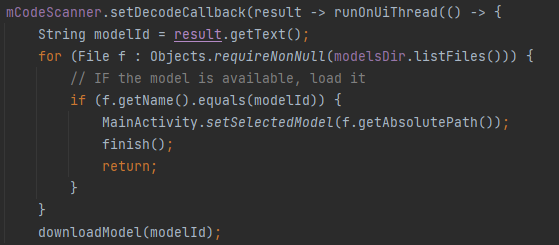
\includegraphics[width=0.5\textwidth]{img/code/loadModelQR.png}}
    \vspace{0.3cm}
    \subfigure[downloadModel] {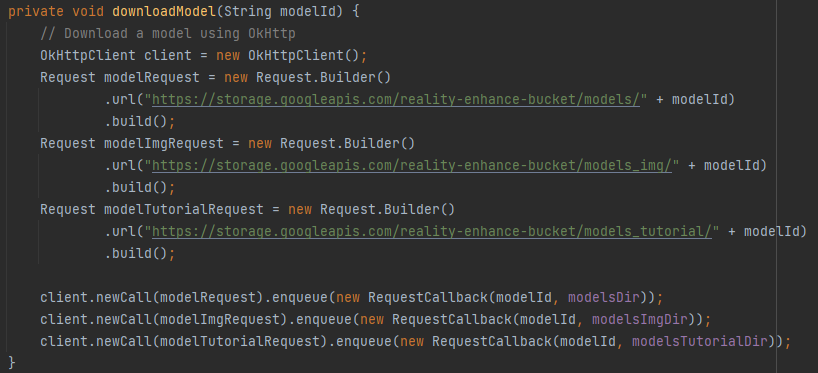
\includegraphics[width=0.5\textwidth]{img/code/downloadModel.png}}
    \caption{QR code-scanner methods}
    \label{fig:loadModelQR}
\end{wrapfigure}



Then the application will handle the response from the Google Bucket Storage. If the response is successful, the model will be saved in the local models directory and loaded in the \ac{AR} scene. If the response is not successful, the application will display an error message, as seen in Figure \ref{fig:onResponse}.


\begin{wrapfigure}{l}{.45\textwidth}
    \centering
    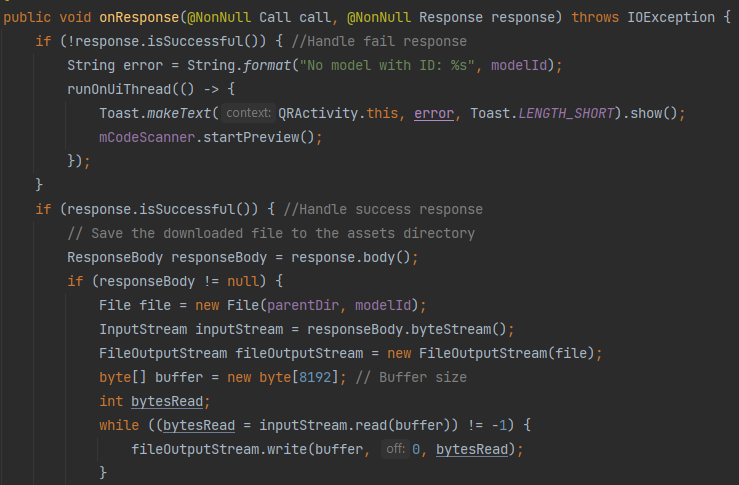
\includegraphics[width=0.45\textwidth]{img/code/onResponse.png}
    \caption{onResponse method}
    \label{fig:onResponse}
\end{wrapfigure}

\clearpage

\section{Load the starting models}
When the user starts the application, the method from Figure \ref{fig:tryMoveAssets} will be called.
\begin{figure}[H]
    \centering
    \subfigure{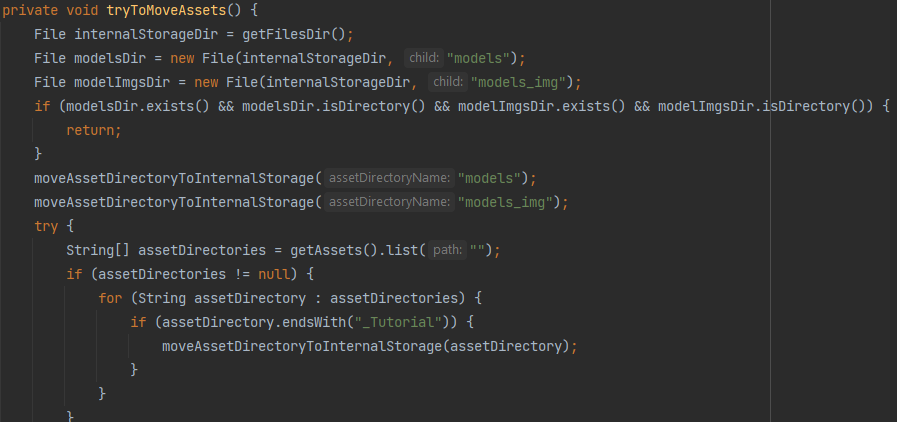
\includegraphics[width=0.8\textwidth]{img/code/tryMoveAssets.png}}
    \subfigure{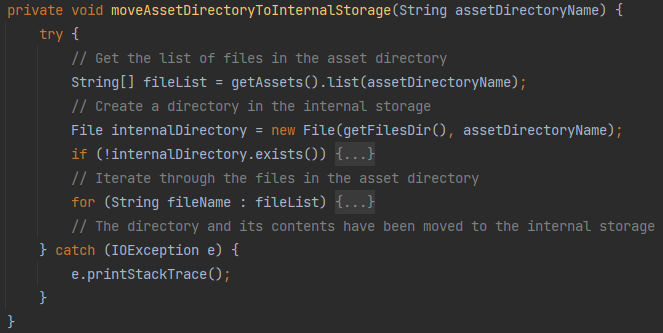
\includegraphics[width=0.6\textwidth]{img/code/moveAssets.png}}
    \caption{Move files from assets to local storage}
    \label{fig:tryMoveAssets}
\end{figure}


It will load the models from the assets directory to the local smartphone storage, because the assets directory is read-only at runtime and the application must store all the newly imported models at the same location. The method will check if the models are already in the local storage. If they are, it will load them from there. If they are not, it will copy them from the assets directory to the local storage.

\newpage
\section{Models' library}
In the Library Activity, the models will be displayed on two columns. This is done at the start of the activity, in the method from Figure \ref{fig:loadModels}. It will go through all the files from the local models directory and it will create a new button for each file.

The buttons will have as background the image of the model. If the model does not have a background image, the button will have as background the name of the model. When the user clicks on a button, the model will be loaded in the \ac{AR} scene.

\begin{figure}[H]
    \centering
    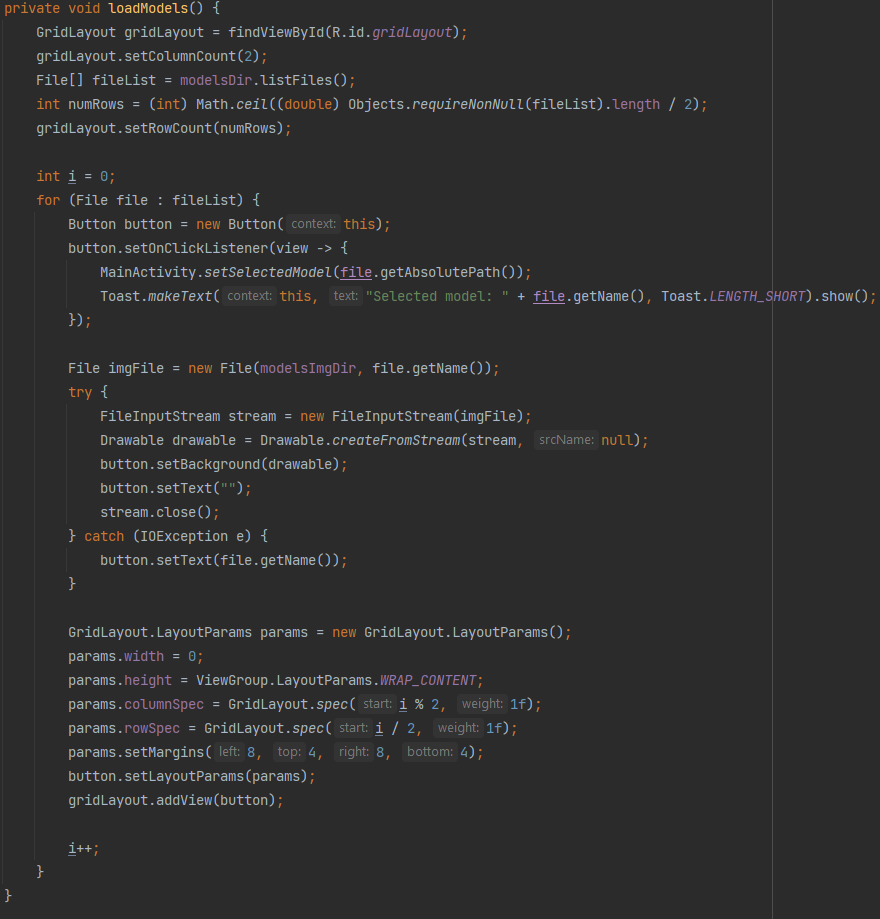
\includegraphics[width=0.8\textwidth]{img/code/loadModels.png}
    \caption{Load models in the library}
    \label{fig:loadModels}
\end{figure}

\newpage
\section{Interaction with  the models}
The user can interact with the models in the \ac{AR} scene by using the buttons on the screen and using smart gestures on the model. As seen in Figure \ref{fig:addModeltoScene}, when the user taps on the screen the addModelToScene method will be called. It will check if the model has a interactive mode, if it does, it will activate the button responsible for the interaction with the model. If the model does not have an interactive mode, it will display a message to the user. Each time the user presses the interaction button, the model will change its state.

\begin{figure}[H]
    \centering
    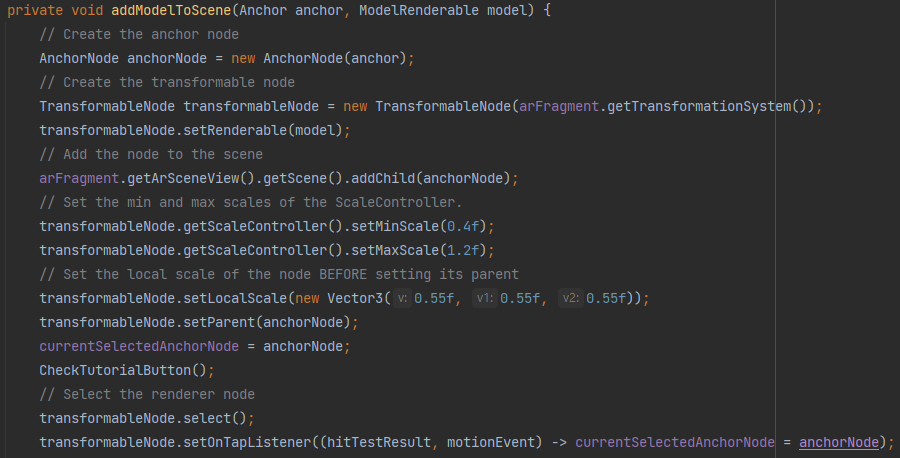
\includegraphics[width=0.8\textwidth]{img/code/addModelToScene.png}
    \caption{addModelToScene method}
    \label{fig:addModeltoScene}
\end{figure}

If a model is selected and the user wants to remove that model from the scene, he can do that by pressing the remove button. This will call the removeAnchorNode method, as seen in Figure \ref{fig:removeAnchorNode}. It will remove the model from the scene and it will set the selectedModel variable to null.

\begin{figure}[H]
    \centering
    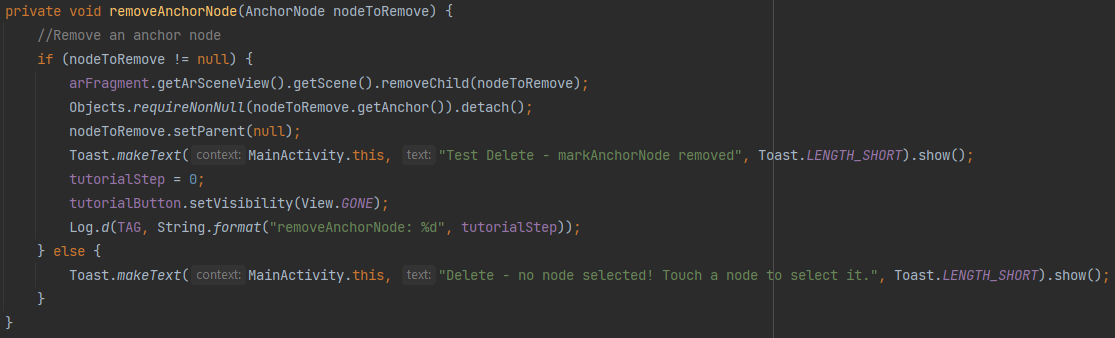
\includegraphics[width=1\textwidth]{img/code/removeAnchorNode.png}
    \caption{removeAnchorNode method}
    \label{fig:removeAnchorNode}
\end{figure}